\section{补充数据与实验图}\label{app:results}
四份数据分别用于房价、收入、得分和成绩预测。表中列出文件规模和观测单位。
\begin{table}[!htbp]\centering\small
\begin{tabularx}{\textwidth}{lrrYY}
\toprule
数据 & 行数 & 列数 & 观测单位 & 默认目标\\
\midrule
房价 & 1,460 & 81 & 一条房屋交易记录 & 成交价\\
Adult & 48,842 & 15 & 一条人口特征记录 & 年收入是否超过 5 万美元\\
NBA & 12,844 & 22 & 一条姓名与赛季表现记录 & 场均得分\\
学生成绩 & 1,000 & 8 & 一条课程样本记录 & 数学成绩\\
\bottomrule
\end{tabularx}
\end{table}
Adult 数量包含原始训练和测试文件，NBA 列数包含导出的行索引。四份表分别分析。数据来源见 \citet{house}、\citet{adult}、\citet{nba} 和 \citet{student}。
\source{\code{tables/data_profile.csv}；\code{data/manifest.json}}

十二个配置在模型拟合前写入本地协议。八个主配置对应四份数据各两个算法，另外四个配置改变房价与 NBA 的划分方式。各配置固定超参数和随机种子，保留大误差记录。输入特征和样本划分见正文表~\ref{tab:sample}。

\subsection{房价预测}
房价主配置的验证误差见图~\ref{app:fig:house}。相同的六个输入变量下，线性回归的 $R^2$ 为 0.8267，随机森林为 0.8527。房价未取对数，四条居住面积超过 4,000 平方英尺的记录保留，极端误差也计入 RMSE。
\begin{figure}[!htbp]\centering
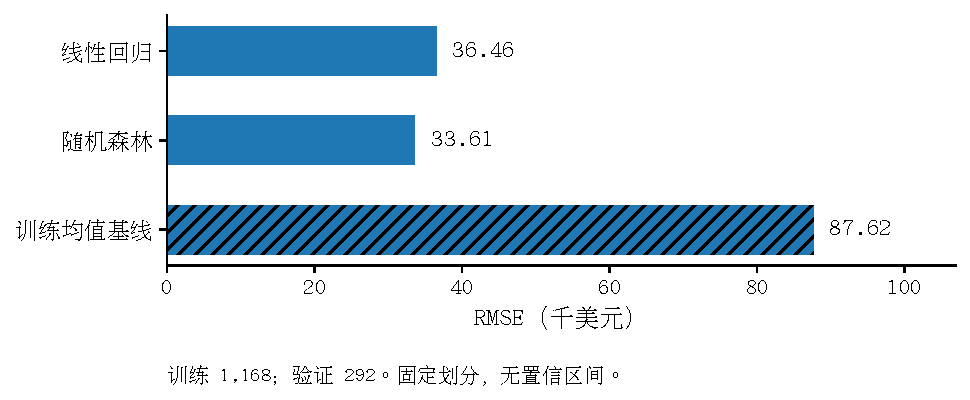
\includegraphics[width=.86\textwidth]{figures/house_rmse_slide.pdf}
\caption{房价主配置的验证误差。横轴为千美元，数值越小越好。}
\label{app:fig:house}
\end{figure}
\subsection{球员得分}
NBA 的跨赛季验证误差见图~\ref{app:fig:nba}。验证数据出现六个训练时未见的选秀年份类别，编码为全零，并记录提示。模型没有学习过这些类别的独立系数。按姓名分组与按赛季留出的结果见正文表~\ref{tab:scores}。
\begin{figure}[!htbp]\centering
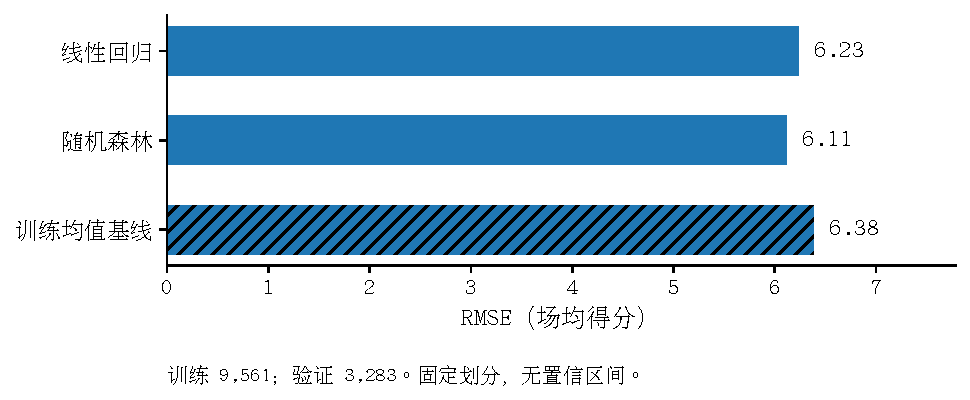
\includegraphics[width=.86\textwidth]{figures/nba_rmse_slide.pdf}
\caption{NBA 后六个赛季共 3,283 条记录的验证误差。单位为场均得分。}
\label{app:fig:nba}
\end{figure}
\subsection{学生成绩}
学生数学成绩的验证误差见图~\ref{app:fig:students}。线性回归和森林的 MAE 分别为 11.453 与 11.502 分。两者使用相同的四个考前背景字段。
\begin{figure}[!htbp]\centering
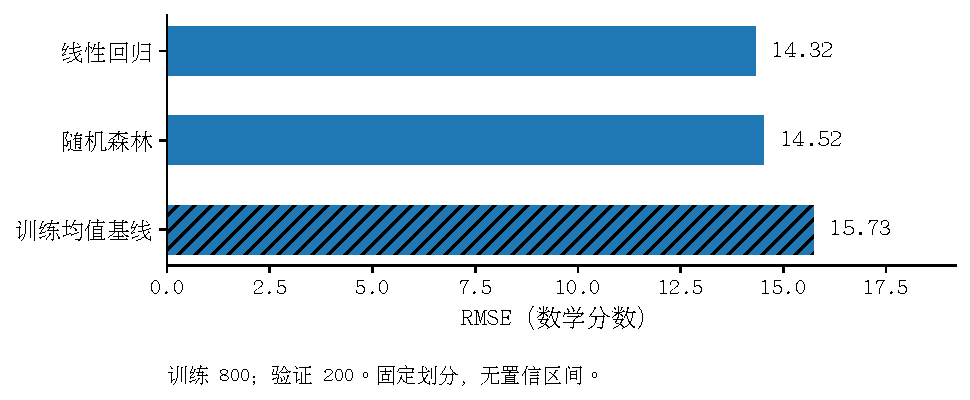
\includegraphics[width=.86\textwidth]{figures/students_rmse_slide.pdf}
\caption{使用四个背景字段预测数学成绩，验证样本为 200 条。同期阅读、写作分数未作为输入。}
\label{app:fig:students}
\end{figure}
\FloatBarrier
收入分类验证集的正类比例约为 24.08\%。训练正类比例作为常数概率时，Brier 分数为 0.1828；两个模型的结果见正文表~\ref{tab:adult}。误报和漏报的用途及成本影响模型选择，本次比较固定使用 0.5 阈值。

十二个配置的全部数值保存在原 CSV 中，包括准确率、平衡准确率、平均精确率和改变划分方式后的结果。本文使用可查看、可重复计算的验证样本，最终盲测尚未开展。
\source{\code{tables/model_comparison.csv}；\code{tables/metric_reconciliation.csv}}
